% !TEX root = ../main.tex

\section{Result}



In the chorus effect, when you compare the 2 sound clips the one before the chorus affect is added and the one after.
You notice a more smoothness of tone and the sound of extra trumpets especially jumps out at you which really gives the appearance of grandeur.
the difference can also be seen visually by inspecting figure \ref{fig:monkeyIslandchorus} and \ref{fig:monkeyIsland} which shows the signal before and after chorus effect was added.

\begin{figure}[!hbt]
	\centering
	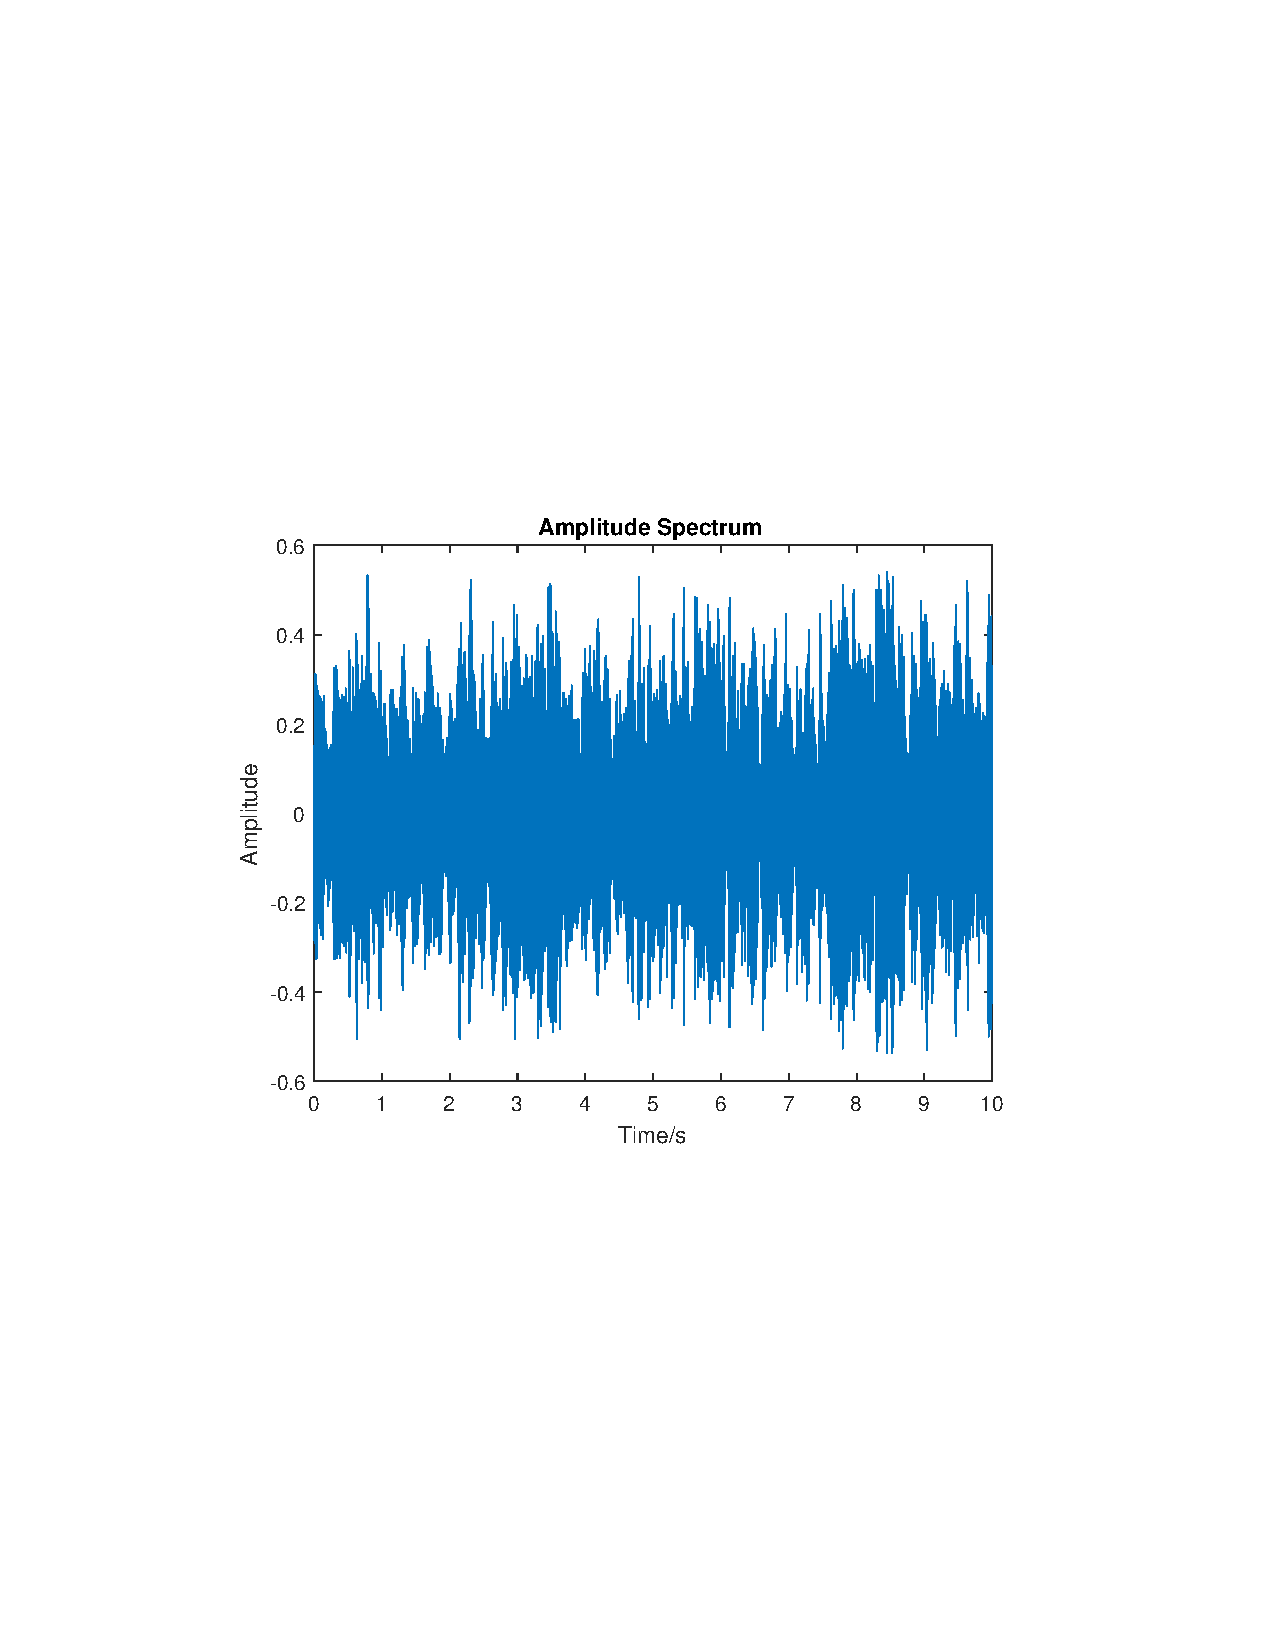
\includegraphics[width=\textwidth]{monkeyIslandchorus.pdf}
	\caption{Excerpt of the theme from Monkey Island in the time domain, with the chorus effect added .}
	\label{fig:monkeyIslandchorus}
\end{figure}
